
\newcommand{\param}[2]{\textit{#1}\,--\,#2\,--\,}
\newcommand{\paramnott}[2]{#1\,--\,#2\,--\,}

\chapter{Praktická část}
Praktická část práce se skládá z~dvou častí. První část je implementace samotného protokolu L2RS a~druhá část je ukázková aplikace která využívá implementaci protokolu. Sekce níže popisují jednotlivé části práce.

\section{Protokol L2RS}
Protokol L2RS je implementovaný v jazyku Python a jako jedinou knihovnu využívá \texttt{numpy}. Parametre pro protokol bili zvolené následovně
\begin{itemize}
  \item \param{q}{12289}modulus pre koeficienty v polynomech,
  \item \param{n}{512}počet koeficientů v polynomech,
  \item \param{m}{6}počet polynomů vo vektoru polynomů,
  \item \paramnott{$\sigma$}{283754}standardní guassova odchylka,
  \item \paramnott{$\gamma$}{13.6}hustota privátního klíče.
\end{itemize}
Tyto parametre bily zvolené aby splňovali bezpečnostní úroveň \texttt{III} protokolu. Vytváření podpisu trvá průměrně 43\,ms a ověření průměrně 38\,ms při výše opomenutých parametrech. Rychlost podpisu a ověření je samozřejmé závislá na parametrech stroje na kterém byli testované. Tyto časy byli měřené na procesoru AMD Ryzen 3600 z frekvencí jádra 3.6\,GHz.

V tabulce \ref{sizes} je možné vidět velkosti jednolitých konstrukcí jako veřejný nebo~privátní klíč. Velkosti podpisu jsou lineárně závislé na počtu uživatelů který se zúčastňují podpisu. Velkost podpisu se dá jednoduše vypočítat podle rovnice
\begin{equation}
  S=1792+w*m*896
\end{equation}
kde $w$ označuje počet uživatelů a $m$ je počet polynomech ve jedním vektoru polynomu.

\begin{table}[htbp]
  \centering
  \caption{Velkosti konstrukcí podpisu}
  \begin{tabular}{|l|c|c|}
    \hline
    Typ              & Počet uživatelů & Velkost (B) \\
    \hline
    Veřejný klíč     & -               & 896         \\
    Privátní klíč    & -               & 4480        \\
    Veřejný parametr & -               & 8960        \\
    Podpis           & 1               & 7168        \\
    Podpis           & 2               & 12544       \\
    Podpis           & 5               & 28672       \\
    \hline
  \end{tabular}
  \label{sizes}
\end{table}


\section{Ukázková aplikace}
Součást práce je taktéž ukázková aplikace která vyváří komunikaci mezi uživateli který jsou schopný ověřovat vytvořené podpisy. Aplikace se skládá z třech částí: \textbf{proxy server}, \textbf{podpisovatel} a \textbf{ověřovatel}. Jako je možné vidět na obrázku \ref{network_diagram}, proxy server přeposílá generovaný podpis všem připojeným ověřovatelům. Taky se~stará o~generovaní veřejných parametrů které posílá na vyžádaní uživatelům. Uživatel může být ověřovatel nebo podpisovatel. 

Podpis se generuje jenom jedním podpisovatelem z využitím soukromého klíče, veřejných parametru a veřejných klíčů všech účastníku. Veřejné klíče jsou zasílané uživateli proxy serveru když se poprvé připojí a vygenerují si soukromý a veřejný klíč. Proxy server stejně jako veřejné parametre poskytuje i posbírané veřejné klíče na vyžádaní. Když podpisovatel zašle vygenerovaný podpis na správu která byla zadaná, je přeposlána všem uživatelům aby ji mohly ověřit pomocí veřejných parametru, veřejných klíčů všech účastníku a originální správy.

\begin{figure}[htbp]
  \centering
  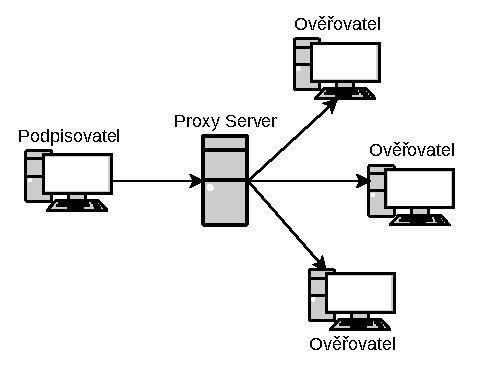
\includegraphics[width=0.65\textwidth]{img/network_diagram.pdf}
  \caption{Sítová komunikace}
  \label{network_diagram}
\end{figure}

Stanice si mezi sebou správy vyměňují pomocí protokolu TCP s jednoduchou aplikační hlavičkou, který formát je možné vidět na obrázků \ref{header}. Políčko \texttt{typ} správy označuje co je obsahem správy. Typy správ jsou následovné:
\begin{itemize}
  \item \texttt{NEED\_PUB\_PARAMS} -- uživatel požaduje veřejné parametre,
  \item \texttt{PUB\_PARAMS} -- server posílá veřejné parametre,
  \item \texttt{MY\_PUB\_KEY} -- uživatel zasílá svůj veřejný klíč,
  \item \texttt{NEED\_PUB\_KEYS} -- uživatel požaduje veřejné klíče všech uživatelů,
  \item \texttt{PUB\_KEYS} -- server posílá veřejné klíče všech uživatelů,
  \item \texttt{SIGNATURE} -- uživatel nebo server zasílá podpis na ověření.
\end{itemize}

\begin{figure}[htbp]
  \centering
  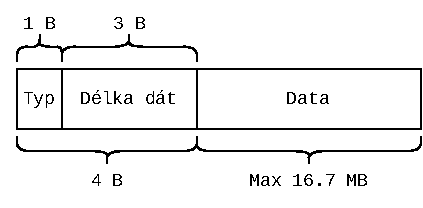
\includegraphics[width=0.7\textwidth]{img/header.pdf}
  \caption{Aplikační hlavička}
  \label{header}
\end{figure}

\subsection{Návod na použití}
Program používá přepínače na jeho ovládaní. Spuštění je možné ve Windows powershellu, WSL (Windows Subsystem for Linux) a libovolné linux distribuci. Program byl testovaný na verzi \texttt{Python 3.10.7}. Návod na spuštění je následovný. Jako první je potřeba nainstalovat potřebné balíčky pomocí souboru \texttt{requirements.txt} který se nachází v odevzdaném kódu:
\begin{itemize}
  \item \texttt{pip install -r requirements.txt}
\end{itemize}
Spustit \textbf{pouze jeden} proxy server:
\begin{itemize}
  \item \texttt{./ring\_sig.py -sp}
\end{itemize}
Spustit \textbf{pouze jednoho} podpisovatele:
\begin{itemize}
  \item \texttt{./ring\_sig.py -c -s}
\end{itemize}
Spustit \textbf{maximum 255} ověřovatelů:
\begin{itemize}
  \item \texttt{./ring\_sig.py -c -v}
\end{itemize}
Dále stačí jednom zadat text který bude podepsaní a ověřený u každého ověřovatele. Jako předvolené nastavení používá program port \textbf{3000} pro komunikaci. Tento port je možné změnit pomocí přepínače \texttt{-p}.
\begin{itemize}
  \item \texttt{./ring\_sig.py -p [PORT]}
\end{itemize}
Všechny dostupné přepínače se dají zobrazit pomocí:
\begin{itemize}
  \item \texttt{./ring\_sig.py -h}
\end{itemize}
Dále je možné zobrazit jednotlivé parametre které sou použité pro protokol L2RS a~sítovou komunikaci:
\begin{itemize}
  \item \texttt{./ring\_sig.py -i}
\end{itemize}


